\documentclass[12pt,letterpaper]{report}

\marginparsep 0pt
\textwidth 6in
\topmargin 0pt
\headsep .5in
\textheight 9.2in
\voffset = 0pt
\hoffset = 0pt
\marginparwidth = 0pt \oddsidemargin = 0pt \sloppy

%Dimensiones de la página
\usepackage[left=2.5cm,top=2cm,right=2.5cm,bottom=1.5cm]{geometry}
%Sangría
\setlength{\parindent}{1cm}

%Numeracion
\pagenumbering{arabic}

\usepackage[utf8]{inputenc}
\usepackage[spanish]{babel}
\usepackage{graphicx}
\usepackage{graphics}
\usepackage[dvips]{epsfig}
\usepackage[dvips]{graphicx}
\usepackage{rotating}
\usepackage{multirow}
\usepackage{longtable}
\usepackage[]{fontenc}
\usepackage{times}
\usepackage[usenames]{color}
\usepackage{templateICI}
\usepackage{amsmath,amsfonts}
\newcommand{\ie}{i.e.}
\newcommand {\out}[1]{}
\newtheorem{definicion}{Definicion}
\usepackage{array}
\usepackage{hyperref}

\renewcommand{\shorthandsspanish}{}
\addto\captionsspanish{
\def\listtablename{Índice de tablas}
\def\tablename{Tabla}}

\sloppy

\begin{document}
\title{\textbf{Sistema de Minería de Datos para apoyar la toma de decisiones de profesionales que utilizan NCFAS en el PPF AITUÉ}}
\author{\textbf{Marcelo Esteban Verdugo Reyes}}
\principaladviser{Eliana Paz Providel Godoy}
\coprincipaladviser{Nombre Profesor Correferente}
\firstreader{Nombre Profesor Informante 1}

\beforepreface
\prefacesection{Resumen}
En Chile existen diferentes familias que se encuentran en situaciones de riesgo social, el cual repercute, ocasionalmente en vulneraciones de los derechos de los niños, niñas y adolescentes (NNA)\footnote{En las siguientes páginas se utilizará a menudo la sigla NNA para referirse a los niños, niñas y adolescentes.}. Existen distintas instituciones para la protección de los integrantes de las familias, dentro de estas se encuentran las corporaciones que buscan intervenir en ellas con el fin de brindar apoyo en las tareas de crianza y desarrollo personal de los NNA. 
En estas corporaciones los profesionales capacitados utilizan diferentes herramientas para analizar situaciones de riesgo en la cual se ven insertas estas familias, donde la experiencia en la toma de decisiones juega un rol fundamental.\\ 
Estas corporaciones por lo general no disponen de herramientas que utilicen Tecnologías de Informaci\'on y Comunicaci\'on (TIC) por lo cual en este Trabajo de T\'itulo se busca apoyar a los especialistas con herramientas TIC, para as\'i agilizar sus procesos y tambi\'en ser de ayuda a la hora de tomar decisiones.


\renewcommand{\thepage}{\roman{page}}
\tableofcontents
\newpage
\listoftables
\listoffigures
\newpage

%Aqui deben incluir el fuente de cada capitulo, sin su encabezado.
\renewcommand{\thepage}{\arabic{page}}
\chapter{Introducción}
\label{intr}
\vspace{2mm}
\normalsize


Uno de los derechos fundamentales de los niños, niñas y adolescentes es que sus necesidades sean satisfechas para desarrollarse y alcanzar la madurez. 
Esta tarea, principalmente recae en los padres y cuidadores, pero además de ellos, también se ven involucrados el conjunto de la sociedad en la que se encuentran los NNA. Por lo cual es necesario que cada adulto, cada comunidad y cada Estado disponga de los cuidados, la protección y la educación que estos necesitan para llegar a la adolescencia y luego a la vida adulta, de una forma sana, constructiva y feliz\cite{REF1}. \\

Está demostrado\cite{REF2} que los trastornos del desarrollo, comportamientos agresivos y violentos, así como otras manifestaciones negativas de los NNA, tienen una estricta relación cuando estos son víctimas y testigo de violencia en el ámbito familiar. Por lo cual es necesario prevenir los malos tratos infantiles para evitar desencadenar estas conductas negativas. Por ejemplo en la región de Valparaíso, comuna de Viña del Mar, específicamente en la población Forestal, se puede observar que la población infanto juvenil se caracterizan por ser víctimas de maltrato y negligencia, agresiones verbales, físicas y/o descalificaciones de mayor o menor gravedad. Entre los niños y niñas de edad preadolescente se observa bajos niveles de autoestima y percepción de logros; recurrentes problemas conductuales, malos tratos a nivel familiar y de pares, ausentismo y riesgo de deserción escolar y bajo rendimiento académico. Entre la población adolescente es posible observar conducta sexual precoz y/o de riesgo, conflictos delictuales, uso de alcohol y/o drogas, embarazo precoz, deserción escolar, micro tráfico,  falta de proyectos de vida, entre otros \cite{REF3}.\\

Por estos motivos nacen diferentes corporaciones que tienen por labor proteger los derechos de los NNA, uno de ellos es la Corporación Comunidad la Roca que trabaja con un proyecto llamado Programas de Prevención Focalizada (PPF Aitué) que es una de las redes colaboradoras del SENAME, que se ubica en la población de Forestal Alto en Viña del Mar. Este proyecto tiene por objetivo que los niños, niñas y adolescentes fortalezcan sus recursos personales, autoestima, auto imagen y habilidades sociales. Junto con ello, que los adultos responsables cuenten con las herramientas y oportunidades para el ejercicio de una parentalidad positiva y que las familias cuenten con apoyos para favorecer la crianza y el desarrollo de los niños, niñas y adolescentes. \\

El proyecto PPF Aitué utiliza diferentes herramientas al momento de trabajar con las familias y los NNA.
Cuando los NNA son derivados al centro (Por el TRIFAM, CESFAM, colegio, etc), primero que todo se realiza un análisis de la situación actual familiar. Para esto el profesional se dirige al hogar de NNA con el fin de poder observar las condiciones en la que él y su familia conviven, además realiza entrevistas para que posteriormente con la información obtenida, el profesional logre formar un juicio del funcionamiento familiar actual.\\

Posteriormente se utiliza una herramienta llamada NCFAS la cual permite ordenar y calificar la apreciación del profesional con respecto a la familia. Con esta apreciación realizada los profesionales logran determinar cuando es necesario intervenir en la familia con el fin de prevenir la vulneración de los derechos de los NNA; o bien para prevenir vulneraciones futuras.\\
Este proceso actualmente se realiza en papel y además, los profesionales no cuentan con una herramientas automatizadas que los apoye en la toma de decisiones.



\chapter{Introducci�n}
\label{intr}

Esta secci�n debe presentar una introducci�n al �rea de trabajo.
Debe introducir terminolog�a b�sica del �rea y principales conceptos
que permitan definir el problema. Aqu� tambi�n debe explicar claramente su aporte.
 Debe haber un p�rrafo explicando la estructura del escrito.
Extensi�n sugerida  es de \textbf{2 p�ginas}.


\chapter{Marco Referencial}
\label{marco}


Los contenidos del informe se definen seg�n el tipo de
trabajo (desarrollo, investigaci�n u otro). El presente documento expone
los contenidos m�nimos exigidos para los cap�tulos \emph{Marco
Referencial} y \emph{Definici�n del problema}. Estos cap�tulos son
obligatorios. No obstante, es el profesor gu�a qui�n debe aprobar la
organizaci�n definitiva de cada uno de ellos seg�n el inter�s del
trabajo. Se debe resguardar la calidad y confiabilidad de las
fuentes bibliogr�ficas. (Este es un ejemplo de como referenciar \cite{khan2014,agrawal94,beeferman00,bharat97}. M\'as ejemplos \cite{dawson}. Para m\'as detalle, revise el archivo \textit{template.bib})

\newpage
\section{Trabajos de T�tulo de Desarrollo}

\subsection{Marco conceptual}

\subsubsection{Definici�n del �rea del problema} \label{contexto}
\vspace{2mm}
\normalsize
Situar el problema en un �rea espec�fica del conocimiento. definir
terminolog�a b�sica del �rea. Referenciar trabajos y resultados
fundamentales. Extensi�n sugerida de \textbf{4 p�ginas}.

\vspace{2mm}

\subsubsection{T�cnicas y herramientas existentes}
\label{tec}

\vspace{1mm}

\normalsize

Revisar sistemas similares, herramientas relacionadas y/o proyectos
relacionados a su trabajo. Resuma las contribuciones e ideas
centrales de cada herramienta relacionada en no m�s de media p�gina
por cada una. Su extensi�n m�xima es de \textbf{7 p�ginas}.

\vspace{2mm}

\subsubsection{Comparaci�n entre ellas} \label{comp}

\vspace{1mm}

\normalsize

Defina y priorice criterios de comparaci�n seg�n el inter�s del
problema. Incluya un cuadro comparativo de las herramientas indicando
su idea central, fortalezas y debilidades. Si existe una
categorizaci�n de ellas, debe incluirla en esta secci�n. Su
extensi�n m�xima es de \textbf{2 p�ginas}.

\vspace{3mm}
\section{Trabajos de T�tulo de Investigaci�n}


\subsection{Marco Referencial}
\label{marco}

\subsubsection{Definiciones}

\vspace{1mm}

\normalsize

Incluya definiciones de conceptos y terminolog�a b�sica del �rea.
S�lo incluya lo necesario para despu�s poder presentar su problema.
Referencie autores con contribuciones originales y relevantes al
�rea. Su extensi�n m�xima es de \textbf{5 p�ginas}.

\vspace{2mm}

\subsubsection{Estado del arte}

\vspace{1mm}

\normalsize

Revise la literatura e incluya trabajos relacionados. Referencia
s�lo aquellos trabajos relevantes a su problema. Clasifique los
trabajos. Puede usar una clasificaci�n estandar de su �rea. Su
extensi�n m�xima es de \textbf{10 p�ginas}.

\vspace{2mm}

\subsubsection{Comparaci�n entre trabajos relacionados}

\vspace{1mm}

\normalsize

Incluya un cuadro comparativo de los trabajos relacionados
definiendo fortalezas y debilidades de cada uno. Su extensi�n m�xima
es de \textbf{3 p�ginas}.

\vspace{3mm}
\normalsize
\chapter{Definici�n del Problema y An�lisis}
\section{Trabajos de T�tulo de Desarrollo}

\label{definicion}
\subsection{Definici�n del problema} \label{prob}

\vspace{1mm}

\normalsize

Redefina el problema que present� en su propuesta incluyendo
\textbf{todas} las observaciones que se le hicieron tanto al informe
escrito como a la presentaci�n oral que realiz�. Precise prop�sito y
metodolog�a. Incluya las siguientes secciones.

\vspace{1mm}

\subsection{Sistema actual}

\vspace{1mm}

\normalsize

En esta secci�n debe entregarse una s�ntesis de la definici�n y especificaci�n de requerimientos. S�lo deben incluirse en �l, los modelos principales. El detalle de los modelos debe entregarse en anexos. Al especificar los requerimientos debe verificar que estos sean necesarios, no ambiguos, trazables, factibles de ser medidos y probados, completos, consistentes y deben estar debidamente priorizados.

Descripci�n del sistema actual: �mbito, prop�sito, objetivos, usuarios, modos de operaci�n, etc. Su extensi�n m�xima es de \textbf{3 p�ginas}.

\subsection{Naturaleza del cambio}

\vspace{1mm}

\normalsize

Identifique, Describa la naturaleza del cambio que introducir�. Su extensi�n
m�xima es de \textbf{2 p�ginas}.

\vspace{1mm}

\subsection{Especificaci�n de requerimientos}

\vspace{1mm}

\normalsize

Descripci�n formal de la soluci�n propuesta (Modos de operaci�n y  An�lisis). Metodolog�a de desarrollo.  Su extensi�n m�xima es de \textbf{15 p�ginas}.


\section{Trabajos de T�tulo de Investigaci�n}
\subsubsection{Definici�n del problema}

\vspace{1mm}

\normalsize

Redefina el problema que present� en su propuesta incluyendo
\textbf{todas} las observaciones que se le hicieron tanto al informe
escrito como a la presentaci�n oral que realiz�. Precise prop�sito y
metodolog�a. Incluya las siguientes secciones.

\vspace{1mm}

\subsubsection{Definici�n del problema}

\vspace{1mm}

\normalsize

Defina formalmente su problema. Defina expl�citamente hip�tesis o lineamientos, preguntas de investigaci�n, y metodolog�a
de investigaci�n.  Use notaci�n matem�tica de ser
necesario. Su extensi�n m�xima es de \textbf{3 p�ginas}.

\vspace{1mm}

\section{Soluci�n propuesta}

\vspace{1mm}

\normalsize

Describa la soluci�n propuesta. Incluya objetivos generales y
espec�ficos. Su extensi�n m�xima es de \textbf{3 paginas}.





\chapter{Definición del Problema y Análisis}
\label{definicion}

\section{Definición del problema} \label{prob}

\vspace{1mm}
\normalsize

Tal como se mencionó en párrafos anteriores, los profesionales del PPF Aitué utilizan herramientas de evaluación, las cuales logran capturan  el funcionamiento familiar.
Para llenar esta escala el profesional realiza visitas domiciliarias y observaciones, donde dicha información permite al profesional formarse un juicio sobre las características del funcionamiento familiar actual. Posteriormente la herramienta permite ordenar esta información y además exige la asignación de puntajes a las diferentes dimensiones que cubre. 
Esta escala (en papel) es llenada manualmente por el profesional lo que permite obtener un puntaje para cada dimensión evaluada. Esta puntuación es analizada para ver si es necesario intervenir o no en la familia evaluada, con el fin de prevenir maltratos infantiles y negligencia parental.\cite{VALENCIA2010}
De acuerdo a lo anterior, se detectan los siguientes problemas:

\begin{itemize}
	\item Falta de un sistema que automatice el proceso de la asignación de puntajes por parte del profesional, para que este, posteriormente pueda realizar la apreciación familiar.
	\item Falta de disposición de información digital de las apreciaciones familiares
	\item Falta de información útil y no trivial para apoyar la toma de decisiones del profesional  
\end{itemize}

\vspace{1mm}

\section{Objetivos}

\vspace{1mm}

\normalsize

En esta sección se explicarán los objetivos generales y los objetivos específicos para lograr el desarrollo del sistema propuesto en el Trabajo de Título.

\subsection{Objetivo General}

El objetivo de este trabajo de título es desarrollar un sistema que automatice la herramienta de apreciación NCFAS y que además, proporcione información útil y no trivial cuando un profesional del PPF Aitué realice una apreciación familiar.

\subsection{Objetivos Específicos}


Para cumplir con el objetivo general es necesario cumplir los siguientes
objetivos específicos:
\begin{itemize}
	
	\item Realizar simulación de datos.
	
	\item Analizar y comparar diferentes técnicas de minería de datos y estadística descriptiva.
	
	\item	Implementar las técnicas de Minería de Datos seleccionada. 
	
	\item	Generar reportes según las técnicas de estadística descriptiva seleccionada. 
	
	\item	Detectar patrones dentro de los descriptores de la herramienta NCFAS, utilizando Minería de Datos. 
	
	
\end{itemize}


\section{Sistema Actual}
\vspace{1mm}
\normalsize

El sistema actual del PPF Aitué para la apreciación familiar utilizando la herramienta NCFAS se puede describir bajo los siguientes pasos:

\begin{itemize}
	\item \textbf{1:} El NNA es derivado al PPF Aitué
	\item \textbf{2:} El asistente social a cargo recopila información necesaria de la familia y del NNA 
	\item \textbf{3:} El profesional utiliza la información recopilada para evaluar la familia utilizando la herramienta NCFAS en papel
	\item \textbf{4:} Obtiene los resultados de la herramienta NCFAS generando un informe
	\item \textbf{5:} De acuerdo al informe se determina el plan de intervención que necesita la familia y el NNA
\end{itemize}

En la Figura \ref{Figura9} se ejemplifica el funcionamiento del sistema actual en el PPF Aitué.



\begin{figure}[htb]
	\label{Figura9}
	\begin{center}
		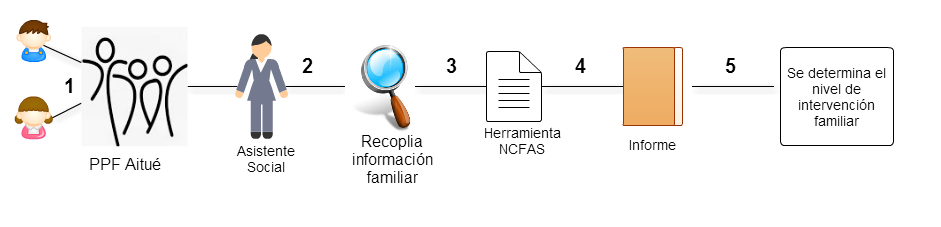
\includegraphics[scale=0.5]{imagenes/diagramancfas.png}
	\end{center}
	\caption{Diagrama del Sistema Actual.}
\end{figure}





\section{Origen del Cambio}
\vspace{1mm}
\normalsize

Con el objetivo de automatizar el sistema actual se propone crear un sistema que permitirá al profesional del PPF Aitué automatizar el proceso de asignación de puntaje por medio de la herramienta NCFAS. Este sistema, además, dispondrá de diferentes módulos (estadística descriptiva y minería de datos), los cuales entregarán al profesional información útil y no trivial para apoyarlo en la toma de decisiones con respecto a la prevención de maltratos infantiles y la negligencia parental. 
Cabe mencionar que para la realización de este sistema sólo se utilizarán datos simulados validados por los profesionales. 

\subsection{Producto}
\vspace{1mm}
\normalsize

Los productos que se obtendrán tras el desarrollo del presente Trabajo de Título son los siguientes:
\begin{itemize}
	\item Un sistema de minería de datos para el apoyo de los profesionales que trabajan con  NCFAS en el PPF Aitué
	\item Manual de usuario
	\item Documentación del análisis del requerimientos ( Especificación de requerimientos) y documentación del diseño para la escalabilidad del sistema
	\item Informe final del Trabajo de Título donde se encontrará detallado el desarrollo del sistema.
\end{itemize}

\subsection{Impacto}
\vspace{1mm}
\normalsize

Con el apoyo de este sistema el profesional, al realizar una nueva apreciación familiar podrá:
\begin{itemize}
	\item Realizar el proceso de manera más eficiente.
	\item Encontrar información útil y no trivial para obtener apoyo a la hora de tomar decisiones, lo cual permitirá realizar un mejor proceso de prevención de maltratos y negligencia parental.
	\item Mejorar el cumplimiento de los profesionales con respecto plazos establecidos para la apreciación familiar. 
\end{itemize}

\section{Especificación de Requerimientos}
\vspace{1mm}
\normalsize

\subsection{Definición de requerimientos}
\vspace{1mm}
\normalsize
En esta sección se presentan los requerimientos para la realización del sistema de apoyo para los profesionales del PPF Aitué. Estos requerimientos se clasificarán en requerimientos funcionales y no funcionales. 

\subsubsection{Requerimientos funcionales}
A continuación se presentan los requerimientos funcionales los cuales se identificarán por la sigla RF.

\begin{itemize}
	\item \textbf{RF1:} Creación de usuarios del sistema con sus respectivos perfiles 
	\item \textbf{RF2:} Digitalización de la herramienta NCFAS
	\item \textbf{RF3:} Creación de un repositorio de las apreciaciones realizadas por los profesionales
	\item \textbf{RF4:} Creación de un módulo de minería de datos
	\item \textbf{RF5:} Creación de un módulo de comparación entre las apreciaciones de ingreso y egreso de la familia
	\item \textbf{RF6:} Creación de un módulo de estadística descriptiva
	\item \textbf{RF7:} Creación de un módulo de búsqueda de las apreciaciones realizadas 
\end{itemize}

\subsubsection{Requerimientos no funcionales}

A continuación se presentan los requerimientos funcionales los cuales se identificarán por la sigla RNF.

\begin{itemize}
	\item \textbf{RNF8:} El sistema debe proveer al usuario de una interfaz usable
	\item \textbf{RNF9:} El sistema debe soportar S.O Windows 7 en adelante 
	\item \textbf{RNF10:} El sistema debe proveer seguridad, ya que se trabajará con datos sensibles
	\item \textbf{RNF11:} El sistema debe proveer ayuda para agilizar el proceso de apreciación ( Mostrar descriptores de los ítems de NCFAS)
	\item \textbf{RNF12:} La interfaz debe ser amigable y contener imágenes representativas para la NCFAS
\end{itemize}

En la Tabla \ref{tablareq} se define la sigla, clasificación y priorización de los requerimientos identificados. A continuación se definen los parámetros utilizados: 

\begin{itemize}
	\item \textbf{Funcional:} El requerimiento expresa la naturaleza del funcionamiento de la plataforma
	\item \textbf{No funcional:} El requerimiento expresa las restricciones de funcionamiento de la plataforma
	\item \textbf{Obligatorio:} El requerimiento se debe desarrollar para el funcionamiento del sistema
	\item \textbf{Necesario:} El requerimiento es requerido pero no imprescindible
	\item \textbf{Prescindible:} El requerimiento se puede dejar de desarrollar y el sistema de igual forma podrá funcionar
\end{itemize}

\begin{table}[h]
\centering
\label{tablareq}
\begin{tabular}{|c|c|l|c|}
	\hline \textbf{Requerimiento} & \textbf{Sigla} & \textbf{Calificación} & \textbf{Prioridad}\\
	\hline 1 & RF1 & Funcional & Obligatorio \\ 
	\hline 2 & RF2 & Funcional & Obligatorio \\ 
	\hline 3 & RF3 & Funcional & Obligatorio \\ 
	\hline 4 & RF4 & Funcional & Obligatorio \\ 
	\hline 5 & RF5 & Funcional & Obligatorio \\ 
	\hline 6 & RNF6 & No Funcional & Obligatorio \\ 
	\hline 7 & RNF7 & No Funcional & Prescindible \\ 
	\hline 8 & RNF8 & No Funcional & Obligatorio \\ 
	\hline 9 & RNF9 & No Funcional & Necesario \\ 
	\hline 10 & RNF10 & No Funcional & Necesario \\ 
	\hline 11 & RNF11 & No Funcional & Prescindible \\ 
	\hline 12 & RNF12 & No Funcional & Prescindible \\
	\hline 
\end{tabular} 
\caption{Tabla Requerimientos del Sistema}
\end{table}

\subsection{Definición de usuarios y tareas del sistema}
El Sistema propuesto diferencia a 2 tipos de usuario, estos son los siguientes: 

\begin{itemize}
	\item \textbf{Administrador:} Usuario con los privilegios necesarios para manejar todos los datos y apreciaciones almacenadas en el sistema.
	\item \textbf{Profesional a cargo:} Usuario encargado de realizar las apreciaciones, además puede utilizar todas las herramientas del sistema (Visualizar información útil y no trivial, buscar apreciaciones anteriores, comparar apreciaciones, etc.)
\end{itemize}
	Para definir el dominio del sistema se definen los siguientes parámetros: 
	
	\begin{itemize}
		\item \textbf{Integro:} Conocimiento total de la plataforma.
		\item \textbf{Esencial:} Conocimiento completo de los módulos utilizados por el profesional a cargo.
	\end{itemize}
	
Además se considera la variable frecuencia de interacción cuyos parámetros son los siguientes: 

\begin{itemize}
	\item \textbf{Alta:} Utilización diaria de la plataforma.
	\item \textbf{Baja:} Utilización mensual o a mayor plazo de la plataforma.
\end{itemize} 

Finalmente se considera para cada tarea de usuario su importancia. Esta variable está determinada con los siguientes parámetros:

\begin{itemize}
	\item \textbf{Crítica:} Cuando la tarea es fundamental para el correcto funcionamiento de la plataforma.
	\item \textbf{Necesaria:} Cuando la tarea afecta sólo a algunos módulos de la plataforma.
	\item \textbf{Intrascendente:} Cuando la tarea es independiente de los demás módulos de la plataforma.
\end{itemize}

\clearpage
\newpage

En la tabla \ref{tareasuser}  se presentan los usuarios y las tareas clasificadas con los parámetros mencionados anteriormente.\\

\begin{table}[h]
	\centering
	\label{tareasuser}
\begin{tabular}{|p{2.5cm}|p{1.5cm}|p{6cm}|p{2cm}|p{2cm}|}
	\hline \textbf{Nivel de Acceso} & \textbf{Dominio del Sistema} & \textbf{Tareas} & \textbf{Importancia}  & \textbf{Frecuencia de Interacción}\\ 
	\hline Administrador & Integro &  Gestionar Usuarios del Sistema & Crítica & Baja \\
	\hline &  & Gestionar NCFAS digital & Crítica & \\
	\cline{3-4}
	Profesional a Cargo & Esencial & Visualizar información útil y no trivial & Necesaria  & Alta\\\cline{3-4} 
	&  & Buscar apreciaciones guardadas & Necesaria & \\ 
	\hline 
\end{tabular} 
\caption{Tabla que presenta las tareas de usuario clasificadas con los parámetros mencionados anteriormente.}
\end{table}

\subsection{Definición de las funciones del sistema}

En esta sección se presentan las funciones que debe ofrecer el sistema propuesto. En la tabla \ref{tablafunc} se asocia un código a cada función.

\begin{table}[h]
\centering
\label{tablafunc}
\begin{tabular}{|c|l|}
	\hline \textbf{Código} & \textbf{Función} \\
	\hline F01 & Crear usuario \\ 
	\hline F02 & Guardar usuario  \\
	\hline F03 & Modificar usuario \\ 
	\hline F04 & Eliminar usuario \\ 
	\hline F05 & Ingresar una apreciación  \\
	\hline F06 & Modificar una nueva apreciación  \\
	\hline F07 & Guardar apreciación \\
	\hline F08 & Buscar apreciaciones guardadas \\
	\hline F09 & Desplegar apreciación guardada\\
	\hline F10 & Desplegar información módulo estadística descriptiva \\ 
	\hline F11 & Desplegar información módulo minería de datos  \\ 
	\hline F12 & Comparar apreciaciones\\
	\hline 
\end{tabular} 
\caption{Tabla Funciones del Sistema}
\end{table}

\subsection{Modelo Conceptual}

En esta sección se presenta el modelo conceptual del sistema. En este se muestran las funcionalidades que realizan las entidades más importantes que componen la totalidad del sistema.
Algunas clases de la Figura \ref{Figura10} tienen palabras abreviadas para facilitar la visualización de la imagen en donde:\\

\begin{itemize}
	\item Modulo E.D representa: Modulo de Estadística Descriptiva.
	
	\item Técnicas E.D representa: Técnicas de Estadística Descriptiva.
	
	\item Módulo M. de D. representa: Módulo de Minería de Datos.
	
	\item Técnicas de M. de D. representa: Técnicas de Minería de Datos. 
\end{itemize}

\begin{figure}[htb]
	\centering
	\label{Figura10}
	\begin{center}
		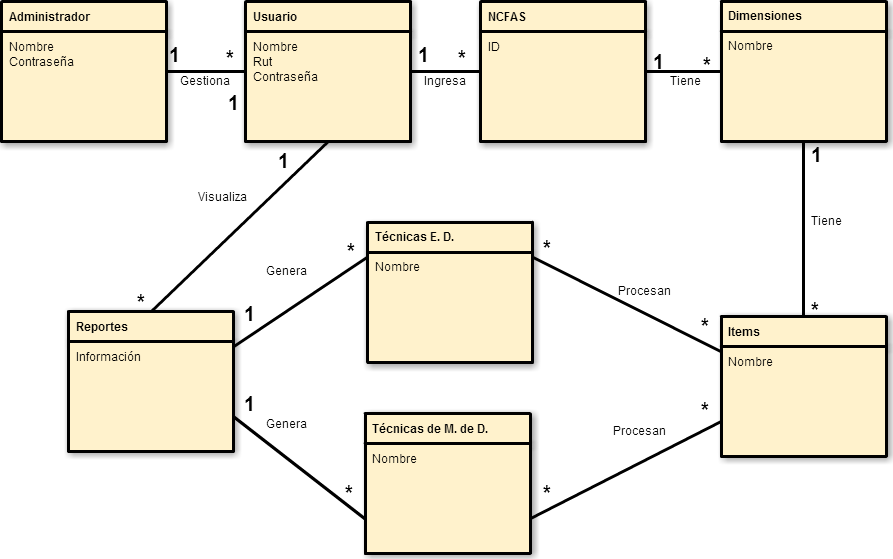
\includegraphics[scale=0.4]{imagenes/Database.png}
	\end{center}
	\caption{Modelo Conceptual del Sistema.}
\end{figure}

\clearpage 	
\newpage

\subsection{Diagrama de Casos de Uso}

En esta sección se representan las funcionalidades del sistema en forma de diagrama de casos de uso. Estos diagramas serán utilizados al momento de desarrollar las diferentes funcionalidades, ya que nos permite observar la comunicación entre ellas y los actores del sistema. La primera figura representa el caso de uso de forma general, y las siguientes figuras representan los casos de uso de manera mas detallada.

\begin{figure}[htb]
	\label{Figura11}
	\begin{center}
		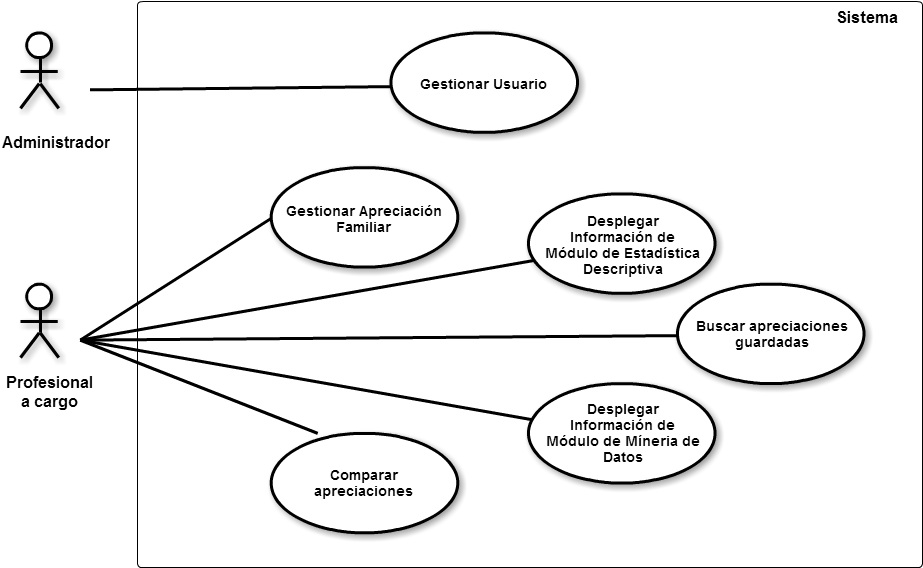
\includegraphics[scale=0.4]{imagenes/diagramacdu.png}
	\end{center}
	\caption{Diagrama de Caso de Uso general.}
\end{figure}

\begin{figure}[htb]
	\label{Figura12}
	\begin{center}
		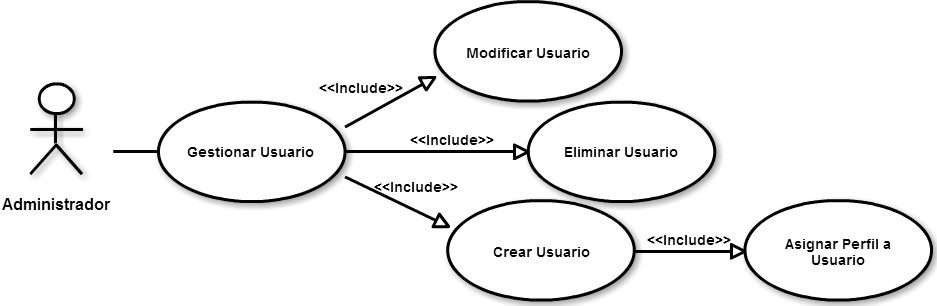
\includegraphics[scale=0.4]{imagenes/CDU1.png}
	\end{center}
	\caption{Caso de Uso Gestionar Usuario.}
\end{figure}


\begin{figure}[htb]
	\label{Figur7}
	\begin{center}
		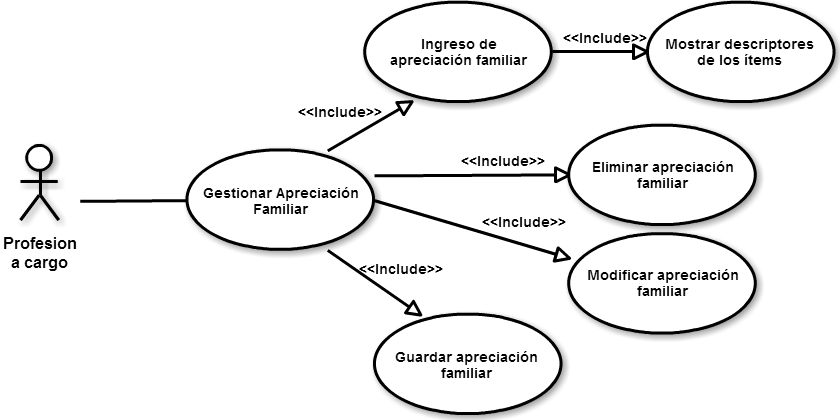
\includegraphics[scale=0.4]{imagenes/CDU2.png}
	\end{center}
	\caption{Caso de Uso NCFAS Digital.}
\end{figure}

\newpage
\clearpage

\begin{figure}[htb]
	\label{Figura13}
	\begin{center}
		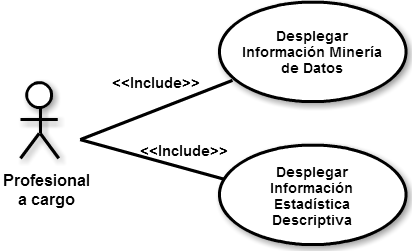
\includegraphics[scale=0.5]{imagenes/CDU3.png}
	\end{center}
	\caption{Caso de Uso Visualizar Información.}
\end{figure}

\begin{figure}[htb]
	\label{Figura14}
	\begin{center}
		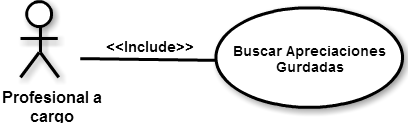
\includegraphics[scale=0.5]{imagenes/CDU4.png}
	\end{center}
	\caption{Caso de Uso Buscar Apreciaciones Guardadas.}
\end{figure}

\begin{figure}[htb]
	\label{Figura15}
	\begin{center}
		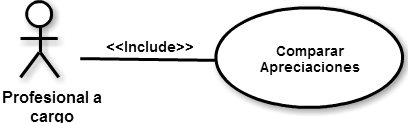
\includegraphics[scale=0.5]{imagenes/CDU5.png}
	\end{center}
	\caption{Caso de Uso Comparar Apreciaciones.}
\end{figure}



\subsection{Caso de Uso en Formato Expandido}
A continuación se presentan los casos de uso en formato expandido, estos explican el proceso de interacción que existe entre el usuario y el sistema detallando cada una de las funciones que tiene el sistema propuesto. 
 
\begin{table}
\centering
\begin{tabular}{|p{6cm} |p{6cm}|}
	\hline \textbf{Caso de Uso} & Crear Usuario  \\ 
	\hline \textbf{ID} & CDU1 \\ 
	\hline \textbf{Actores} & Administrador \\ 
	\hline \textbf{Tipo} & Primario \\ 
	\hline \textbf{Pre-condición} & - \\ 
	\hline \textbf{Descripción} & Permite crear los usuarios del sistema \\
	\hline \textbf{Ref. Cruzadas} & RF1 \\ 
	\hline
	\multicolumn{2}{|c|}{\textbf{Resumen}} \\
	\hline
	\multicolumn{2}{|p{12cm}|}{El administrador crea los usuarios asignando un respectivo nombre de usuario, e-mail, contraseña y perfil para que posteriormente el usuario pueda ingresar al sistema.} \\
	\hline 
\end{tabular}  

\begin{tabular}{|p{6cm}|p{6cm}|}
	
	\multicolumn{2}{|c|}{\textbf{Curso normal de eventos}} \\
	\hline \textbf{Actor} & \textbf{Sistema} \\ 
	\hline 1. Este caso de uso comienza cuando el administrador debe crear un usuario para el sistema. & 2.El sistema solicita al administrador el nombre de usuario, e-mail, contraseña y perfil del nuevo usuario.  \\ 
	3. El administrador ingresa lo solicitado. & 4. El sistema valida lo ingresado por el administrador y crea el nuevo usuario. \\
	 & 5. El sistema guarda el nuevo usuario y permite al administrador crear un nuevo usuario o bien ingresar al sistema. \\
	 \hline
	\multicolumn{2}{|c|}{\textbf{Curso alternativo de eventos}} \\
	\hline
	\multicolumn{2}{|p{12cm}|}{4. El sistema valida los datos ingresados por el administrador pero estos son válidos y vuelve al paso 3.} \\
	\hline
\end{tabular}
\caption{Tabla del caso de uso expandido de Crear Usuario}
\label{tabcdu1}
\end{table}

\newpage
\clearpage
%CASO DE USO EXPANDIDO MODIFICAR USUARIO

\clearpage
\begin{table}
	\centering
	\begin{tabular}{|p{6cm} |p{6cm}|}
		\hline \textbf{Caso de Uso} & Modificar Usuario \\ 
		\hline \textbf{ID} & CDU2 \\ 
		\hline \textbf{Actores} & Administrador \\ 
		\hline \textbf{Tipo} & Opcional \\ 
		\hline \textbf{Pre-condición} & Crear un usuario \\ 
		\hline \textbf{Descripción} & Permite modificar un usuario creado anteriormente \\
		\hline \textbf{Ref. Cruzadas} & RF1 \\ 
		\hline
		\multicolumn{2}{|c|}{\textbf{Resumen}} \\
		\hline
		\multicolumn{2}{|p{12cm}|}{El administrador modifica un usuario creado anteriormente, con la posibilidad de modificar nombre de usuario, e-mail, contraseña o perfil.} \\
		\hline 
	\end{tabular}  
	
	
	\begin{tabular}{|p{6cm}|p{6cm}|}
		
		\multicolumn{2}{|c|}{\textbf{Curso normal de eventos}} \\
		\hline \textbf{Actor} & \textbf{Sistema} \\ 
		\hline 1. Este caso de uso comienza cuando el administrador desea modificar un usuario creado anteriormente, seleccionando la opción modificar usuario. & 2. El sistema muestra los usuarios guardados. \\ 
		3. El administrador selecciona al usuario que desea modificar. & 4. El sistema muestra las opciones a modificar del usuario  \\
		5. El administrador modifica lo necesario. &  \\
		6. El administrador guarda las modificaciones. & 7. El sistema valida las modificaciones y guarda nuevamente el usuario modificado. \\
		\hline
		\multicolumn{2}{|c|}{\textbf{Curso alternativo de eventos}} \\
		\hline
		\multicolumn{2}{|p{12cm}|}{7. El sistema valida los datos ingresados por el administrador pero estos no son válidos y vuelve al paso 5. } \\
		\hline
	\end{tabular}
	\caption{Tabla del caso de uso expandido de Modificar Usuario}
	\label{tabcdu2}
\end{table}

\newpage
\clearpage
%CASO DE USO EXPANDIDO ELIMINAR USUARIO DEL SISTEMA
\clearpage
\begin{table}
	\centering
	\begin{tabular}{|p{6cm} |p{6cm}|}
		\hline \textbf{Caso de Uso} & Eliminar Usuario \\ 
		\hline \textbf{ID} & CDU3 \\ 
		\hline \textbf{Actores} & Administrador \\ 
		\hline \textbf{Tipo} & Opcional \\ 
		\hline \textbf{Pre-condición} & Crear un usuario \\ 
		\hline \textbf{Descripción} & Permite eliminar un usuario creado anteriormente \\
		\hline \textbf{Ref. Cruzadas} & RF1 \\ 
		\hline
		\multicolumn{2}{|c|}{\textbf{Resumen}} \\
		\hline
		\multicolumn{2}{|p{12cm}|}{El administrador elimina un usuario creado anteriormente.} \\
		\hline 
	\end{tabular}  
	\begin{tabular}{|p{6cm}|p{6cm}|}
		\multicolumn{2}{|c|}{\textbf{Curso normal de eventos}} \\
		\hline \textbf{Actor} & \textbf{Sistema} \\ 
		\hline 1. Este caso de uso comienza cuando el administrador desea eliminar un usuario creado anteriormente, seleccionando la opción eliminar usuario. & 2. El sistema muestra los usuarios guardados. \\ 
		3. El administrador selecciona al usuario que desea eliminar. & 4. El sistema envía una alerta para que el administrador confirme que realmente desea eliminar el usuario seleccionado.  \\
		5. El administrador confirma la eliminación. & 6. El sistema elimina al usuario. \\
		\hline
		\multicolumn{2}{|c|}{\textbf{Curso alternativo de eventos}} \\
		\hline
		\multicolumn{2}{|p{12cm}|}{5. El administrador cancela la eliminación del usuario y vuelve al paso 3. } \\
		\hline
	\end{tabular}
	\caption{Tabla del caso de uso expandido de Eliminar Usuario}
	\label{tabcdu3}
\end{table}

\newpage
\clearpage
%CASO DE USO EXPANDIDO INGRESAR NCFAS

\begin{table}
\centering
\begin{tabular}{|p{6cm} |p{6cm}|}
	\hline \textbf{Caso de Uso} & Ingresar una Nueva Apreciación \\ 
	\hline \textbf{ID} & CDU4 \\ 
	\hline \textbf{Actores} & Profesional a cargo \\ 
	\hline \textbf{Tipo} & Primario \\ 
	\hline \textbf{Pre-condición} & - \\ 
	\hline \textbf{Descripción} & Permite ingresar una apreciación familiar por medio de NCFAS Digital \\
	\hline \textbf{Ref. Cruzadas} & RF2 - RF3 - RNF11 \\ 
	\hline
	\multicolumn{2}{|c|}{\textbf{Resumen}} \\
	\hline
	\multicolumn{2}{|p{12cm}|}{El profesional a cargo luego de recopilar la información necesaria de la familia, ordena y califica la información por medio de la herramienta NCFAS Digital.} \\
	\hline 
\end{tabular}  
\begin{tabular}{|p{6cm}|p{6cm}|}
	
	\multicolumn{2}{|c|}{\textbf{Curso normal de eventos}} \\
	\hline \textbf{Actor} & \textbf{Sistema} \\ 
	\hline 1. Este caso de uso comienza cuando el profesional a cargo ingresa una nueva apreciación familiar. & 2. El sistema despliega la herramienta NCFAS Digital.  \\ 
	3. El profesional a cargo califica cada ítem, donde además puede ver los descriptores asociados a cada ítem.&  \\
	4. El profesional guarda todo su progreso. & 5. El sistema guarda y almacena la apreciación completa. \\
	\hline
	\multicolumn{2}{|c|}{\textbf{Curso alternativo de eventos}} \\
	\hline
	\multicolumn{2}{|p{12cm}|}{4. El profesional no guarda la apreciación realizada. } \\
	\hline
\end{tabular}
\caption{Tabla del caso de uso expandido de NCFAS Digital}
\label{tabcdu4}
\end{table}

\newpage
\clearpage
%CASO DE USO EXPANDIDO MODIFICAR NCFAS

\begin{table}
	\centering
	\begin{tabular}{|p{6cm} |p{6cm}|}
		\hline \textbf{Caso de Uso} & Modificar Apreciación \\ 
		\hline \textbf{ID} & CDU5 \\ 
		\hline \textbf{Actores} & Profesional a cargo \\ 
		\hline \textbf{Tipo} & Primario \\ 
		\hline \textbf{Pre-condición} & Existan apreciaciones guardadas \\ 
		\hline \textbf{Descripción} & Permite modificar una apreciación familiar por medio de NCFAS Digital \\
		\hline \textbf{Ref. Cruzadas} & RF2 - RF3 - RF7 RNF11 \\ 
		\hline
		\multicolumn{2}{|c|}{\textbf{Resumen}} \\
		\hline
		\multicolumn{2}{|p{12cm}|}{El profesional luego guardar una apreciación, este, posteriormente puede modificarla.} \\
		\hline 
	\end{tabular}  
	\begin{tabular}{|p{6cm}|p{6cm}|}
		
		\multicolumn{2}{|c|}{\textbf{Curso normal de eventos}} \\
		\hline \textbf{Actor} & \textbf{Sistema} \\ 
		\hline 1. Este caso de uso comienza cuando el profesional a cargo desea modificar una apreciación familiar. & 2.El sistema despliega las apreciaciones guardadas.  \\ 
		3. El profesional a cargo por medio del buscador de apreciaciones, busca cual apreciación desea modificar.& 4. El sistema busca la apreciación a modificar por el profesional a cargo y la muestra. \\
		5. El profesional selecciona la apreciación a modificar. & 6. El sistema despliega la apreciación para modificarla. \\
		7. El profesional modifica lo necesario y guarda los cambios. & 8. El sistema guarda la apreciación modificada. \\
		\hline
		\multicolumn{2}{|c|}{\textbf{Curso alternativo de eventos}} \\
		\hline
		\multicolumn{2}{|p{12cm}|}{7. El profesional modifica pero no guarda los cambios. } \\
		\hline
	\end{tabular}
	\caption{Tabla del caso de uso expandido de Modificar NCFAS Digital}
	\label{tabcdu5}
\end{table}

\newpage
\clearpage
%CASO DE USO EXPANDIDO VISUALIZAR INFORMACIÓN


\newpage
\clearpage
%CASO DE USO EXPANDIDO VISUALIZAR INFORMACIÓN ESTADISTICA

\begin{table}
	\centering
	\begin{tabular}{|p{6cm} |p{6cm}|}
		\hline \textbf{Caso de Uso} & Visualizar Información Estadística Descriptiva \\ 
		\hline \textbf{ID} & CDU6 \\ 
		\hline \textbf{Actores} & Profesional a cargo \\ 
		\hline \textbf{Tipo} & Opcional \\ 
		\hline \textbf{Pre-condición} & Existan apreciaciones guardadas \\ 
		\hline \textbf{Descripción} & Permite que el profesional a cargo visualice información con técnicas de Estadística Descriptiva \\
		\hline \textbf{Ref. Cruzadas} & RF4 - RF6 \\ 
		\hline
		\multicolumn{2}{|c|}{\textbf{Resumen}} \\
		\hline
		\multicolumn{2}{|p{12cm}|}{El profesional a cargo podrá visualizar la información , mediante técnicas de estadística descriptiva.} \\
		\hline 
	\end{tabular}  
	\begin{tabular}{|p{6cm}|p{6cm}|}
		\multicolumn{2}{|c|}{\textbf{Curso normal de eventos}} \\
		\hline \textbf{Actor} & \textbf{Sistema} \\ 
		\hline 1. Este caso de uso comienza cuando el profesional a cargo desea visualizar información mediante el módulo de estadística descriptiva. & 2.El sistema despliega las diferentes técnicas de estadística descriptiva para mostrar la información.  \\ 
		3. El profesional a cargo selecciona una de estas técnicas de estadística descriptiva. & 4.El sistema despliega la información.  \\ 
		\hline
		\multicolumn{2}{|c|}{\textbf{Curso alternativo de eventos}} \\
		\hline
		\multicolumn{2}{|p{12cm}|}{ - } \\
		\hline
	\end{tabular}
	\caption{Tabla del caso de uso expandido de Visualizar Información Módulo Estadística Descriptiva}
	\label{tabcdu6}
\end{table}

\newpage
\clearpage
%CASO DE USO EXPANDIDO VISUALIZAR INFORMACIÓN MINERÍA

\begin{table}
	\centering
	\begin{tabular}{|p{6cm} |p{6cm}|}
		\hline \textbf{Caso de Uso} & Visualizar Información \\ 
		\hline \textbf{ID} & CDU7 \\ 
		\hline \textbf{Actores} & Profesional a cargo \\ 
		\hline \textbf{Tipo} & Opcional \\ 
		\hline \textbf{Pre-condición} & - \\ 
		\hline \textbf{Descripción} & Permite que el profesional a cargo visualice información con técnicas de Minería de Datos \\
		\hline \textbf{Ref. Cruzadas} & RF4 - RF6 \\ 
		\hline
		\multicolumn{2}{|c|}{\textbf{Resumen}} \\
		\hline
		\multicolumn{2}{|p{12cm}|}{El profesional a cargo podrá visualizar información mediante técnicas de minería de datos.} \\
		\hline 
	\end{tabular}  
	\begin{tabular}{|p{6cm}|p{6cm}|}
		\multicolumn{2}{|c|}{\textbf{Curso normal de eventos}} \\
		\hline \textbf{Actor} & \textbf{Sistema} \\ 
			\hline 1. Este caso de uso comienza cuando el profesional a cargo desea visualizar información mediante el módulo de minería de datos. & 2.El sistema despliega las diferentes técnicas de minería de datos para encontrar información útil y no trivial.  \\ 
			3. El profesional a cargo selecciona una de estas técnicas. & 4.El sistema despliega la información.  \\ 
			\hline
			\multicolumn{2}{|c|}{\textbf{Curso alternativo de eventos}} \\
			\hline
			\multicolumn{2}{|p{12cm}|}{ - } \\
			\hline
		\end{tabular}
		\caption{Tabla del caso de uso expandido de Visualizar Información Módulo Minería de Datos}
	\label{tabcdu7}
\end{table}

\newpage
\clearpage
% CASO DE USO EXPANDIDO BUSCAR UNA APRECIACION

\begin{table}
	\centering
	\begin{tabular}{|p{6cm} |p{6cm}|}
		\hline \textbf{Caso de Uso} & Buscar NCFAS Digital \\ 
		\hline \textbf{ID} & CDU8 \\ 
		\hline \textbf{Actores} & Profesional a cargo \\ 
		\hline \textbf{Tipo} & Opcional \\ 
		\hline \textbf{Pre-condición} & EL sistema debe tener NCFAS Digitales almacenados \\ 
		\hline \textbf{Descripción} & Permite buscar una apreciación NCFAS \\
		\hline \textbf{Ref. Cruzadas} & RF2-RF7 \\ 
		\hline
		\multicolumn{2}{|c|}{\textbf{Resumen}} \\
		\hline
		\multicolumn{2}{|p{12cm}|}{El profesional a cargo podrá buscar NCFAS Digitales dentro del sistema.} \\
		\hline 
	\end{tabular}  
	\begin{tabular}{|p{6cm}|p{6cm}|}
		\multicolumn{2}{|c|}{\textbf{Curso normal de eventos}} \\
		\hline \textbf{Actor} & \textbf{Sistema} \\ 
		\hline 1. Este caso de uso comienza cuando el profesional a cargo desea buscar una apreciación familiar. & 2.El sistema despliega un buscador.  \\ 
		3. El profesional a cargo ingresa palabras claves para buscar la apreciación necesaria.& 4. El sistema despliega las NCFAS Digitales correspondientes a la búsqueda del profesional. \\
		\hline
		\multicolumn{2}{|c|}{\textbf{Curso alternativo de eventos}} \\
		\hline
		\multicolumn{2}{|p{12cm}|}{ - } \\
		\hline
	\end{tabular}
	\caption{Tabla del caso de uso expandido de Buscar NCFAS Digital}
	\label{tabcdu8}
\end{table}

\newpage
\clearpage

% CASO DE USO EXPANDIDO COMPARAR APRECIACIONES
\begin{table}
	\centering
	\begin{tabular}{|p{6cm} |p{6cm}|}
		\hline \textbf{Caso de Uso} & Comparar NCFAS Digitales \\ 
		\hline \textbf{ID} & CDU9 \\ 
		\hline \textbf{Actores} & Profesional a cargo \\ 
		\hline \textbf{Tipo} & Opcional \\ 
		\hline \textbf{Pre-condición} & EL sistema debe tener NCFAS Digitales almacenados \\ 
		\hline \textbf{Descripción} & Permite comparar dos NCFAS(Ingreso v/s egreso) \\
		\hline \textbf{Ref. Cruzadas} & RF5 \\ 
		\hline
		\multicolumn{2}{|c|}{\textbf{Resumen}} \\
		\hline
		\multicolumn{2}{|p{12cm}|}{El profesional a cargo podrá comparar NCFAS Digitales dentro del sistema.} \\
		
	\end{tabular}  
	\begin{tabular}{|p{6cm}|p{6cm}|}
		\multicolumn{2}{|c|}{\textbf{Curso normal de eventos}} \\
		\hline \textbf{Actor} & \textbf{Sistema} \\ 
		\hline 1. Este caso de uso comienza cuando el profesional a cargo desea comparar apreciaciones familiares. & 2.El sistema despliega las NCFAS que puede seleccionar para comparar (Las que tengan una apreciación de ingreso y egreso).  \\ 
		3. El profesional a cargo selecciona las NCFAS que desea comparar.& 4. El sistema despliega información acerca de los ítems que más variaron entre el NCFAS de ingreso v/s el NCFAS de egreso. \\
		\hline
		\multicolumn{2}{|c|}{\textbf{Curso alternativo de eventos}} \\
		\hline
		\multicolumn{2}{|p{12cm}|}{ - } \\
		\hline
	\end{tabular}
	\caption{Tabla del caso de uso expandido de Comparar NCFAS Digitales}
	\label{tabcdu9}
\end{table}

\newpage
\clearpage

\subsection{Diagramas de Secuencia}

Los siguientes diagrama de secuencia ilustran gráficamente la interacción entre el usuario y el sistema. \\
A continuación se presentan los diagramas de secuencia para las funciones del sistema.

\begin{figure}[htb]
	\label{dss1}
	\begin{center}
		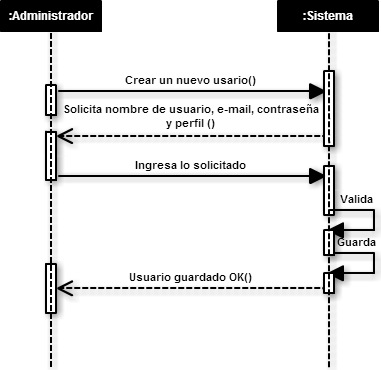
\includegraphics[scale=0.5]{imagenes/creauser2.png}
	\end{center}
	\caption{Diagrama de secuencia: Crear Usuario.}
\end{figure}


\begin{figure}[htb]
	\label{dss2}
	\begin{center}
		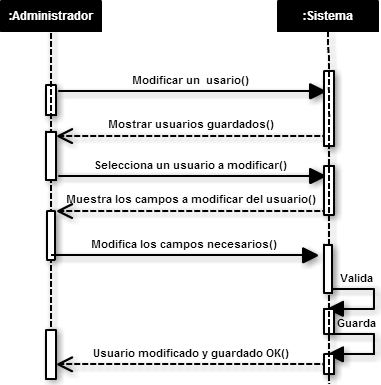
\includegraphics[scale=0.5]{imagenes/modificaruser.png}
	\end{center}
	\caption{Diagrama de secuencia: Modificar Usuario.}
\end{figure}


\begin{figure}[htb]
	\label{dss3}
	\begin{center}
		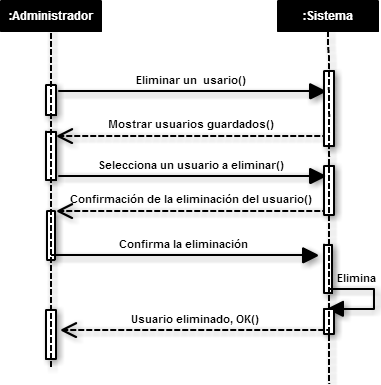
\includegraphics[scale=0.5]{imagenes/eliminaruser.png}
	\end{center}
	\caption{Diagrama de secuencia: Eliminar Usuario.}
\end{figure}


\begin{figure}[htb]
	\label{dss4}
	\begin{center}
		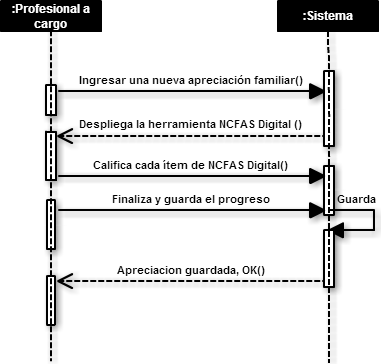
\includegraphics[scale=0.5]{imagenes/ingresarncfas.png}
	\end{center}
	\caption{Diagrama de secuencia: Ingresar Nueva Apreciación.}
\end{figure}


\begin{figure}[htb]
	\label{dss5}
	\begin{center}
		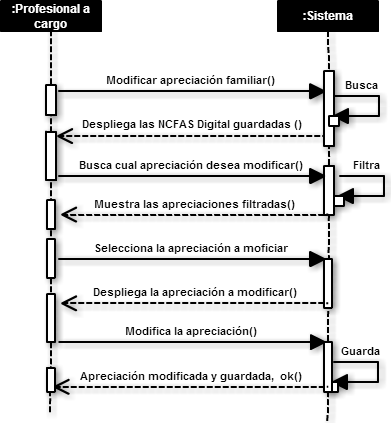
\includegraphics[scale=0.5]{imagenes/modificarncfas.png}
	\end{center}
	\caption{Diagrama de secuencia: Modificar Apreciación.}
\end{figure}


\begin{figure}[htb]
	\label{dss6}
	\begin{center}
		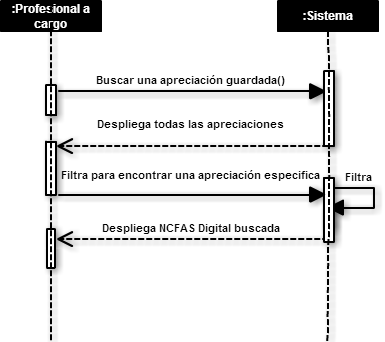
\includegraphics[scale=0.5]{imagenes/buscar.png}
	\end{center}
	\caption{Diagrama de secuencia: Buscar Apreciación.}
\end{figure}

\begin{figure}[htb]
	\label{dss7}
	\begin{center}
		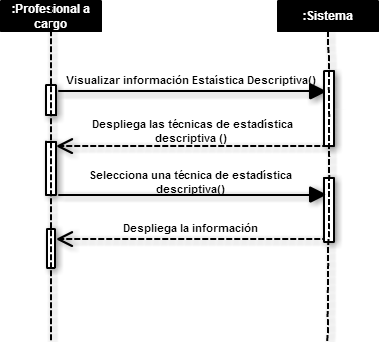
\includegraphics[scale=0.5]{imagenes/visualizared.png}
	\end{center}
	\caption{Diagrama de secuencia: Visualizar Información Estadística Descriptiva.}
\end{figure}


\begin{figure}[htb]
	\label{dss8}
	\begin{center}
		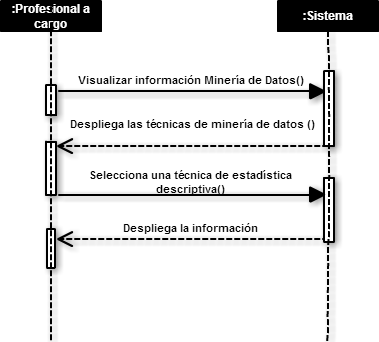
\includegraphics[scale=0.5]{imagenes/visualizarmdd.png}
	\end{center}
	\caption{Diagrama de secuencia: Visualizar Información Minería de Datos.}
\end{figure}

\begin{figure}[htb]
	\label{dss9}
	\begin{center}
		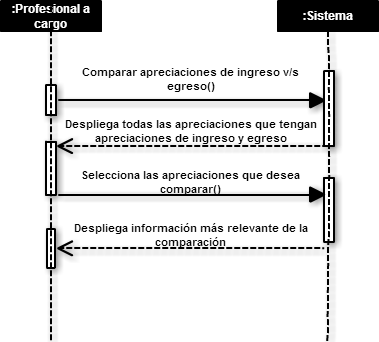
\includegraphics[scale=0.5]{imagenes/comparar.png}
	\end{center}
	\caption{Diagrama de secuencia: Comparar Apreciaciones.}
\end{figure}

\newpage
\clearpage

\subsection{Diagramas de Estado}

Los diagramas de estado presentan los cambios de estado del sistema según se realicen sus funcionalidades. A continuación se presentan los diagramas de estado para las funcionalidades. 

\begin{figure}[htb]
	\label{dde1}
	\begin{center}
		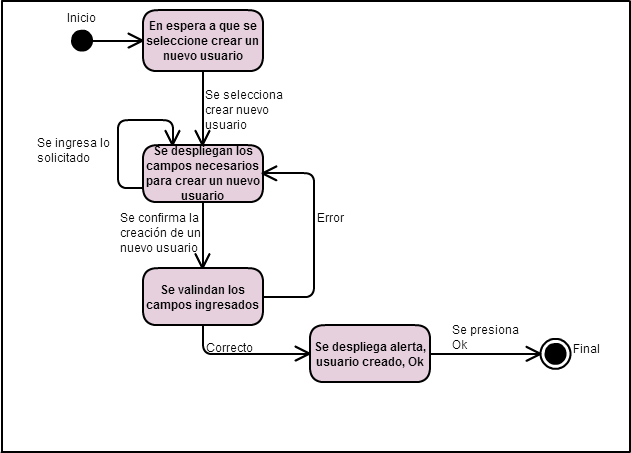
\includegraphics[scale=0.5]{imagenes/crearusuario.png}
	\end{center}
	\caption{Diagrama de estado: Crear Usuario.}
\end{figure}

\begin{figure}[htb]
	\label{dde2}
	\begin{center}
		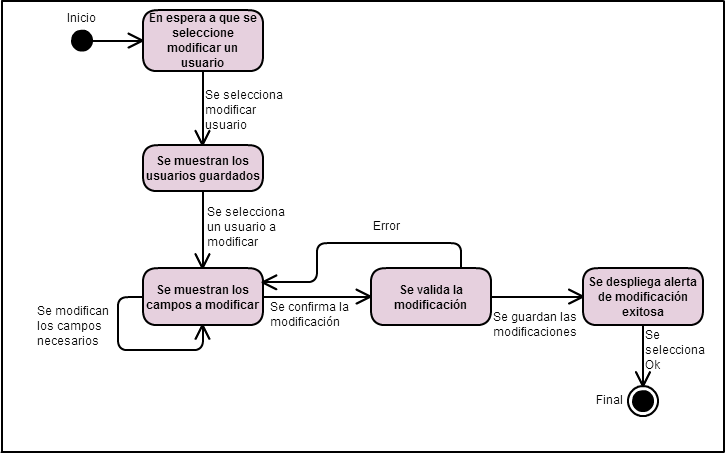
\includegraphics[scale=0.5]{imagenes/ModificarUsuario.png}
	\end{center}
	\caption{Diagrama de estado: Modificar Usuario.}
\end{figure}


\begin{figure}[htb]
	\label{dde3}
	\begin{center}
		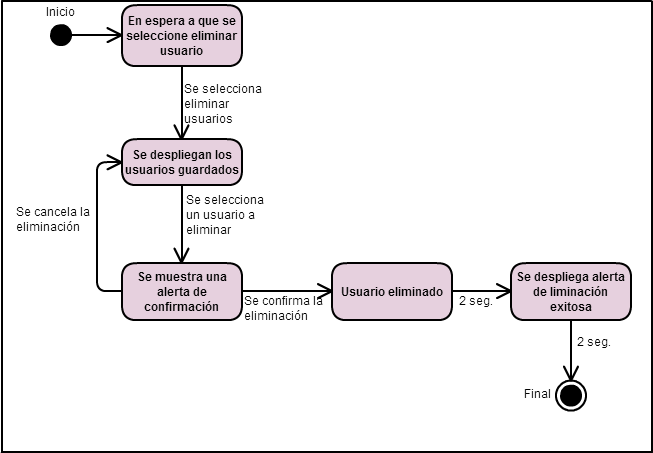
\includegraphics[scale=0.5]{imagenes/EliminarUser2.png}
	\end{center}
	\caption{Diagrama de estado: Eliminar Usuario.}
\end{figure}

\begin{figure}[htb]
	\label{dde4}
	\begin{center}
		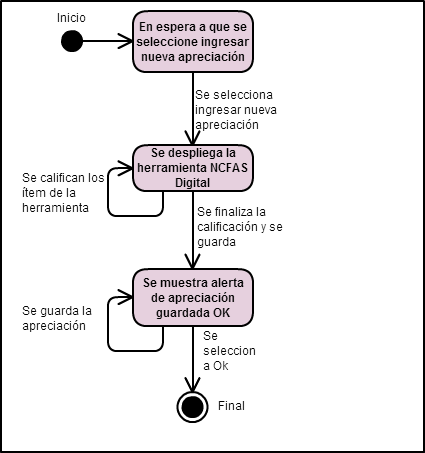
\includegraphics[scale=0.5]{imagenes/IngresarNCFAS2.png}
	\end{center}
	\caption{Diagrama de estado: Ingresar Apreciación.}
\end{figure}


\begin{figure}[htb]
	\label{dde5}
	\begin{center}
		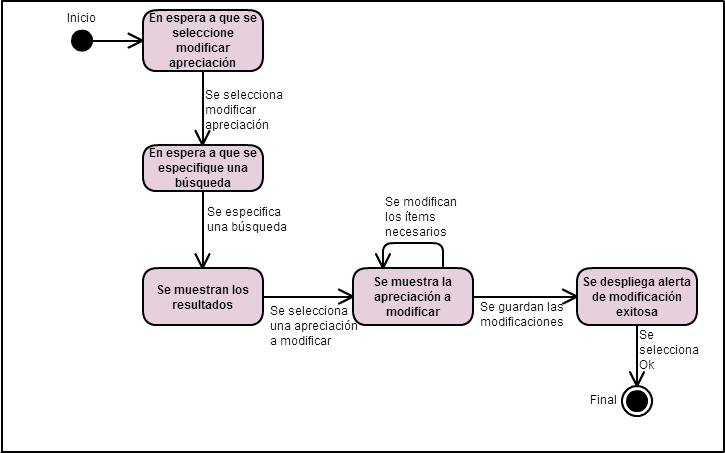
\includegraphics[scale=0.5]{imagenes/ModificarNCFAS2.png}
	\end{center}
	\caption{Diagrama de estado: Modificar Apreciación.}
\end{figure}

\begin{figure}[htb]
	\label{dde6}
	\begin{center}
		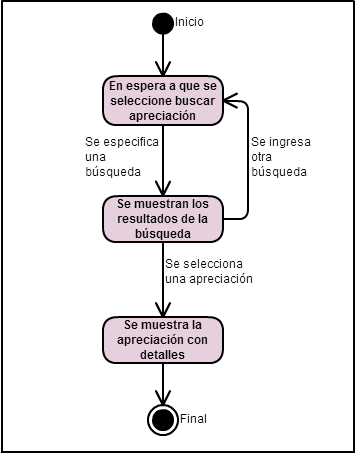
\includegraphics[scale=0.5]{imagenes/BuscarNCFAS.png}
	\end{center}
	\caption{Diagrama de estado: Buscar Apreciación.}
\end{figure}


\begin{figure}[htb]
	\label{dde7}
	\begin{center}
		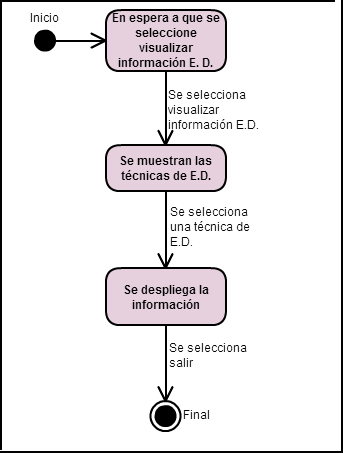
\includegraphics[scale=0.6]{imagenes/VisualizarInfoED.png}
	\end{center}
	\caption{Diagrama de estado: Visualizar Información Estadística Descriptiva.}
\end{figure}

\begin{figure}[htb]
	\label{dde8}
	\begin{center}
		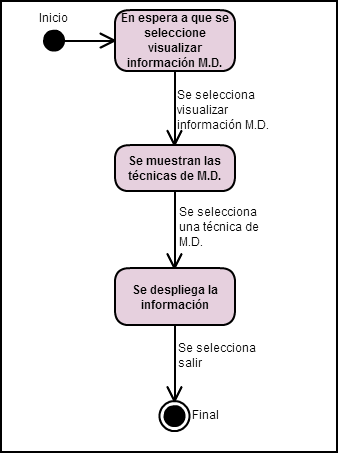
\includegraphics[scale=0.6]{imagenes/VisualizarInfoMD.png}
	\end{center}
	\caption{Diagrama de estado: Visualizar Información Minería de Datos.}
\end{figure}


\begin{figure}[htb]
	\label{dde9}
	\begin{center}
		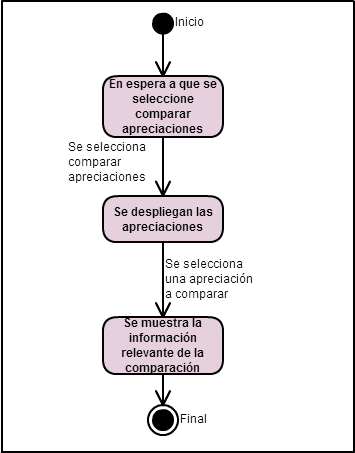
\includegraphics[scale=0.5]{imagenes/compararncfas.png}
	\end{center}
	\caption{Diagrama de estado: Comparar Apreciaciones.}
\end{figure}

\newpage
\clearpage

\section{Conclusión}

En el Capítulo \ref{definicion} se plantea que una herramienta digital de la escala de apreciación NCFAS sería de gran utilidad para los profesionales que trabajan en el PPF Aitué. Además se llevan acabo técnicas de diseño de software para posteriormente apoyar la etapa de desarrollo del sistema propuesto. 


\chapter{Dise�o}
\label{capdiseno}

\section{Introducci�n}

El Informe 3 equivale al cap�tulo de Dise�o de su Trabajo de T�tulo.
 En este documento se describen los contenidos m�nimos exigidos para el Informe 3 y se sugiere la extensi�n (en cantidad de p�ginas) de cada t�pico.
Los contenidos  se definen seg�n el tipo de trabajo que se est� realizando: desarrollo de SW, investigaci�n,  u otro.
 Sin embargo, es el profesor gu�a qui�n debe aprobar su organizaci�n definitiva.
 Tambi�n se debe resguardar la calidad y confiabilidad de las fuentes bibliogr�ficas.

\section{Dise�o Trabajos de T�tulo de Desarrollo de SW}  \label{diseno}
 En este cap�tulo s e describe los contenidos del Cap�tulo de dise�o para los TT de desarrollo de software.
 
 Obs.: Resguardar la trazabilidad y consistencia entre los modelos. Justifique las
decisiones de dise�o.

\subsection{Dise�o arquitect�nico} \label{disenoarq}
Defina (si corresponde) los patrones de dise~no que usar�. Incluya modelo de estructura
del sistema el cual debe reflejar el tipo de arquitectura especifica (cliente-servidor,
3 capas, SOA). Cada m�dulo debe estar trazado con respecto a los subsistemas identificados en el modelo de estructura.
De ser necesario incluya modelo de control.
Extensi�n m�xima sugerida 5 p�ginas.


\subsection{Dise�o de interfaz} \label{disenoint}
Sobre la base del perfil de usuario debe seleccionar el estilo de interacci�n, definir
los objetivos de facilidad de uso, determinar las pautas de estilo. Incluya en anexo el
modelo de navegaci�on. Extensi�n m�xima sugerida 5 p�ginas.

\subsection{Dise�o l�gico} \label{disenolog}
De acuerdo con  la metodolog�a seleccionada, especifique los modelos de dise~no requerido,
por ejemplo para orientaci�n a objeto casos de uso reales (en anexo), diagramas de
colaboraci�n (en anexo) y diagramas de clases. Extensi�n m�xima sugerida 15 p�ginas.


\subsection{Dise�o de datos}  \label{disenodat}
A partir de cada subsistema (consistente con el modelo de estructura del sistema),
definir una componente ER con notaci�n Bachmann. Defina claves candidatas, entidades,
cardinalidades y atributos. Normalice y justifique la normalizaci�n. Integre los
componentes ER en un modelo de datos l�gico interno global Bachmann identificando
claves primarias, for�neas, atributos, tipos de relaciones y cardinalidades. Extensi�n m�xima sugerida 5 p�ginas.


 \subsection{Dise�o de pruebas}

  Debe definir cuidadosamente el objetivo y como realizar� las pruebas de cada parte de su desarrollo:  Pruebas de requerimientos, Pruebas de an�lisis,  Pruebas de dise�o, Pruebas de unidad, Pruebas de integraci�n. Pruebas de sistema. Pruebas de aceptaci�n del usuario, entre otras.


\subsection{Conclusiones}  \label{conclusiones}
Incluya an�lisis cr�tico sobre  pertinencia del problema, soluci�n propuesta, proyecciones
y estado de avance. Extensi�n m�xima sugerida 2 p�ginas.




\section{Dise�o para Trabajos de T�tulo de Investigaci�n}
\label{diseno}
En este cap�tulo s e describe los contenidos del Cap�tulo de dise�o para los TT de Investigaci�n
\subsection{Dise�o de la soluci�n} \label{disenosol}
Defina brevemente el contexto de la soluci�n propuesta. Luego defina detalladamente
la soluci�n. Para esto debe incluir modelos o diagramas descriptivos globales
y luego incluir informaci�n detallada sobre cada m�dulo. En el caso de definici�n de
modelos, se deben incluir variables a considerar y la relaci�n entre estas. Justifique
su dise�o sea riguroso(a).

 Si su soluci�n incluye el desarrollo de algun SW tambi�n debe realizar el dise�o del mismo, de acuerdo a la pauta anterior.
   Extensi�n m�xima sugerida de 15 p�ginas.


\subsection{Dise�o de experimentos} \label{disenoexp}
Defina los  experimentos que debe realizar para responder sus preguntas de investigaci�n.
Cada experimento  debe precisar objetivo, escenarios posibles,
variables involucradas, medidas con las que se trabajar�, pre-experimentos si es
necesario, relaci�n entre las variables (hip�tesis), herramientas y pasos del an�lisis.

 En el caso que los experimentos est�n encadenados, incluya un diagrama de causalidad de
experimentos.  Extensi�n m�xima sugerida de 15 p�ginas.

Obs: lea cuidadosamente los documentos sobre dise�o de experimentos \cite{inv,dawson,fundibeq,extracto_dawson}. Siga la pauta mostrada en las ppt de dise�o de experimentos \cite{extracto_dawson_ppt}.

\subsection{Conclusiones} \label{conclusiones}
Incluya an�lisis cr�tico, pertinencia del problema, soluci�n propuesta, proyecciones
y estado de avance. Extensi�n m�xima sugerida  2 p�ginas.


\section{Dise�o para otros tipos  Trabajos de T�tulo }

 Para TT distintos a los explicados anteriormente deber�n considerar las secciones que  les acomoden, en  acuerdo con su profesor gu�a.
  Si su soluci�n incluye el desarrollo de algun SW tambi�n debe realizar el dise�o del mismo, de acuerdo a la pauta anterior.
 

\bibliographystyle{plain}
\bibliography{informe,terminologia}

\end{document} 